In this chapter the proposed Jacobian controller is experimentally verified. The experimental set-up will first be further detailed. This includes the data acquisition from the sensors. Then experimental results will be shown for a set-point regulation.  


\section{Experimental set-up}

The experimental set-up consisting of the planar soft robot, air pumps, airtanks, and pressure sensors are connected as followed. Each air pump is attached to an air distribution manifold via a hose. This distribution manifold has three air outlets. To these outlets a pressure sensor, air tank and actuator bellow is attached, respectively. To this end, air hoses with a inner diameter of 3mm are used. To the tip of the actuator a yellow LED used for optical tracking is mounted. This LED is glued to a 
connector that has been additively manufactured. The LED has an offset of 45 mm with respect the tip of the actuator. This connector part also houses the Inertial Measurement Unit (IMU). This IMU is used to measure  rotation of the actuator's tip in radians. Furthermore, a vision system is focused on the actuator. This vision system is programmed such it can recognise and track the LED marker. 

The sensors described above, e.g. the IMU, two pressure sensors and optical tracking system are connected to an Arduino micro. This Arduino is then connected to a Raspberry PI 3B+. The Arduino code is programmed such that it constantly updates all sensors. For the optical tracking system, which is the Pixy V2 the update rate is 60 Hz. The pressure sensors and IMU are read at 200 Hz. Once the Raspberry requests sensor data, the Arduino puts a string with delimiters into the Arduino serial. The Raspberry reads this string, separates the sensor data based on this delimiters, and updates the sensor data. This communication allows to reach a sampling frequency of 25 Hz. It would be more convenient to connect the sensors directly to the Raspberry. However, the Raspberry was not able to interpret this sensor data correctly. On this Raspberry the controller was programmed. To this Raspberry a ADC converter shield is mounted which can regulate the pwm input to the air pumps. The programming language used for the Raspberry is C++. For coding on the Arduino, the Arduino language is used. 

Since the position data collected by the vision system contains high-frequent noise, a first order low-pass filter was implemented on the Raspberry. This discrete low-pass filter with a cut-off frequency of 1 Hz and a sample rate of 25 Hz is given as,

\begin{equation}
    Y_k = 0.78Y_{k-1} + 0.22y_k,
\end{equation}

where $Y_k$ is new sensor value, $Y_{k-1}$ previous sensor value. And $y_k$ the new sensor data input. Notice that a zero order hold integration method is used for determining the new sensor value.

On the IMU a complementary filter was introduced. This filter combines gyroscopic data with acceleration data, since a gyroscope is prone to drift. Combining both allows to retrieve more accurate angle data. 


\hl{include complementary filter IMU, low-pass filter on the vision system.}

\subsection{Simplified Inverse Kinematics}

Since the configuration of the actuator is approximated with a single shape function. The inverse kinematic problem can implicitly be solved with the constant curvature approach. The sensor output, which is the x,y position in the plane, and the orientation of the tip of the actuator $\theta$ can be used to determine modal coordinates $\epsilon$ and $\kappa$. At each sampling instant this inverse kinematics are determined. Based on the modal coordinates the Jacobian matrix can be updated, which in its turn is used in determining the new control input. The simplified kinematics are shown in Figure \ref{fig:simpkin}.

\begin{figure}[H]
    \centering
    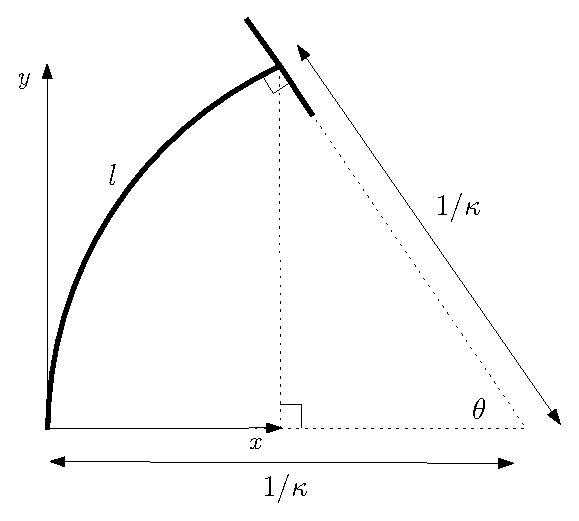
\includegraphics[width = 0.5\textwidth]{Figures/Chapter5/fbdkinematics.eps}
    \caption{Schematic drawing of the actuator to determine mapping from configuration space to task space}
    \label{fig:simpkin}
\end{figure}

From above figure the following forward kinematic relations follow as,


\begin{equation}
    y = \frac{1}{\kappa}\sin(\theta) \hspace{15pt} \text{and} \hspace{15pt}    x = \frac{1}{\kappa}[1-\cos(\theta)] \hspace{15pt} \text{with} \hspace{10pt}   \theta = l \kappa.
\end{equation}

where $l \in \mathbb{R}^{+}$ is the actuator length given by $l = (1+\epsilon)L_0$. Accordingly, the modal coordinates can then be calculated by,

\begin{equation}
    \kappa_y = \frac{\sin(\theta)}{y} \hspace{15pt} 	\land \hspace{15pt}  \kappa_x = \frac{1 -\cos(\theta)}{x} \hspace{15pt} \text{and} \hspace{10pt} \epsilon = \frac{\theta}{\kappa L_0} -1,
\end{equation}

where it should be noted that for small angles it is more accurate to use $\kappa_y$.

\section{Experimental Resutls}





%\textbf{Assumptions}
%\begin{itemize}
%    \item The actuator is symmetrical, curvature equal but negative in when bellow is pressurized
%    \item Out of plane motion is negligible small
%    \item Constant curvature approach captures the kinematics well when neglecting the effect of gravity 
%\end{itemize}



